\documentclass[11pt]{article}
\usepackage[margin=1in]{geometry}
\usepackage{graphicx}
\usepackage{booktabs}
\usepackage{amsmath}
\usepackage{hyperref}
\usepackage{float}
\usepackage{caption}
\usepackage{xcolor}
\usepackage{microtype}
\hypersetup{colorlinks=true, urlcolor=blue!60!black, linkcolor=black}
\captionsetup{font=small, labelfont=bf}
\graphicspath{{../results/}{../results/3d/}}
\newcommand{\code}[1]{\texttt{#1}}
\newcommand{\dB}{\,\mathrm{dB}}
\newcommand{\todo}[1]{\textcolor{red}{\textbf{TODO:} #1}}

\title{A2: Gaussian Splatting}
\author{Zeke Barnett \\ 15-474}
\date{October 2026}

\begin{document}
\maketitle

\noindent\textbf{AI Disclosure:} I used AI to help write parts of the code and to debug when my training runs were getting stuck and seemed like they would never finish. I also used AI to help make the figures for the writeup and write some tests. \\

\noindent\textbf{Code:} \todo{\url{https://github.com/zeke13dev/15-474-A2}}. The repository README gives the commands that regenerate every number and figure below.

\medskip
\noindent\textbf{Setup.} PSNR uses $\mathrm{MAX}=1$ on float images. The 2D targets are the provided $256\times256$ images resized to $128\times128$ (Lanczos); every 2D fit uses the P3 initialization with a fixed seed, Adam at lr $10^{-2}$, and 2000 steps of full-image MSE. The 3D fits use the provided $160\times160$ views, Adam at lr $10^{-2}$, and 1500 steps with one random training camera per step. All runs are on an M-series Mac (\code{mps}).

\paragraph{Renderer.} Compositing follows the handout: Gaussians sorted front to back, $C=\sum_i T_i\alpha_i c_i$ with $T_i=\prod_{j<i}(1-\alpha_j)$, computed for all Gaussians at once with an exclusive \code{cumprod} instead of a Python loop. The first, fully dense version (every pixel against every Gaussian) needed about $1.25$\,s per step at $N=4096$, so a single P5 run took 40 minutes. Following the handout's suggestion, the final renderer cuts the image into $16\times16$ tiles and composites each tile only against the Gaussians whose $3.5\sigma$ bounding box overlaps it. This is about $20\times$ faster ($0.06$\,s per step at $N=4096$, two minutes per run). Contributions beyond $3.5\sigma$ (weight $<0.0022$) are dropped; a unit test checks the tiled renderer against a dense reference with the same cutoff, and the cutoff moved coffee at $N=256$ from $26.16$ to $26.15\dB$.

\section*{P4. Densification}

\paragraph{Rule.} Every 200 steps, until 75\% of training (step 1500), I run a pass. The score $g_i$ is the mean norm of $\partial L/\partial \mu_i$ over the steps since the last pass. I measure it in normalized device coordinates (the pixel gradient times $W/2$, $H/2$), which are the 3DGS paper's units, so the threshold does not depend on image resolution; with raw pixel gradients the paper's $2\times10^{-4}$ selected nothing (the 99th percentile was about $6\times10^{-5}$). Gaussians with $g_i > 10^{-4}$ are densified. I lowered the threshold from the paper's $2\times10^{-4}$ because $g_i$ shrinks as the fit improves, and at $2\times10^{-4}$ growth stopped at 788 of a 1024 budget on astronaut.
\begin{itemize}
\item \emph{Clone} if the Gaussian's largest scale is at most 2\% of the image width (2.6\,px): an exact copy is appended. The copy sits at a different place in the compositing order, so the two receive different gradients and separate.
\item \emph{Split} otherwise: the parent is replaced by two children whose centers are sampled from the parent's own distribution, $\mu + RS z$ with $z\sim\mathcal{N}(0,I)$, with scale divided by $1.6$ and the parent's rotation, color, and opacity.
\item \emph{Prune} Gaussians with opacity below $0.005$.
\item \emph{Budget}: each clone or split adds exactly one Gaussian, so after pruning, at most (budget $-$ count) candidates are densified, highest $g_i$ first.
\end{itemize}
New tensors are swapped into Adam after every pass: survivors keep their moment estimates and new Gaussians start from zero. A densified run starts from $N/4$ Gaussians. In 2D, pruning never fired: from the single viewpoint every Gaussian is visible, so the optimizer has no reason to make one transparent.

\begin{figure}[H]
\centering
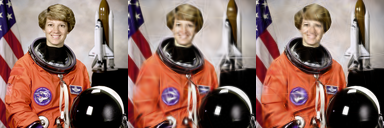
\includegraphics[width=0.75\textwidth]{p4_compare.png}
\caption{Astronaut at $128\times128$. Left to right: target, fixed-count fit with 1024 Gaussians ($27.47\dB$), densified fit grown from 256 to 1024 Gaussians ($\mathbf{29.88\dB}$).}
\label{fig:p4}
\end{figure}

\paragraph{Densified vs.\ fixed.} On astronaut, with both runs ending at exactly 1024 Gaussians, densification reaches $29.88\dB$ against $27.47\dB$ for the fixed-count fit, a $2.4\dB$ gain (Figure~\ref{fig:p4}): the flag stripes, mission patches, and the helmet and shuttle edges are visibly sharper. With a fixed count, the Gaussians mostly stay near their uniformly random starting positions (at lr $10^{-2}$ a center moves at most about $0.01$\,px per step), so smooth regions get as many Gaussians as edges. Densification puts new Gaussians where the gradient says the fit is failing, which is along the edges. Densified runs are also faster, since they spend most of training below the budget. Densified runs at other budgets are on the dashed curves of Figure~\ref{fig:p5}; most of them stopped short of their budget, which I discuss there.

\section*{P5. Quality vs.\ number of Gaussians}

\begin{table}[H]
\centering
\begin{tabular}{lrrr}
\toprule
target & $N=256$ & $N=1024$ & $N=4096$ \\
\midrule
coffee    & 26.15 & 31.88 & 38.21 \\
astronaut & 21.65 & 27.47 & 36.93 \\
cat       & 27.38 & 31.56 & 40.72 \\
\midrule
values stored ($9N$) / raw ($128^2\cdot 3$) & 0.047 & 0.19 & 0.75 \\
\bottomrule
\end{tabular}
\caption{Final PSNR (dB) of fixed-count fits. Same initialization and seed for every run; only $N$ changes.}
\label{tab:p5}
\end{table}

\begin{figure}[H]
\centering
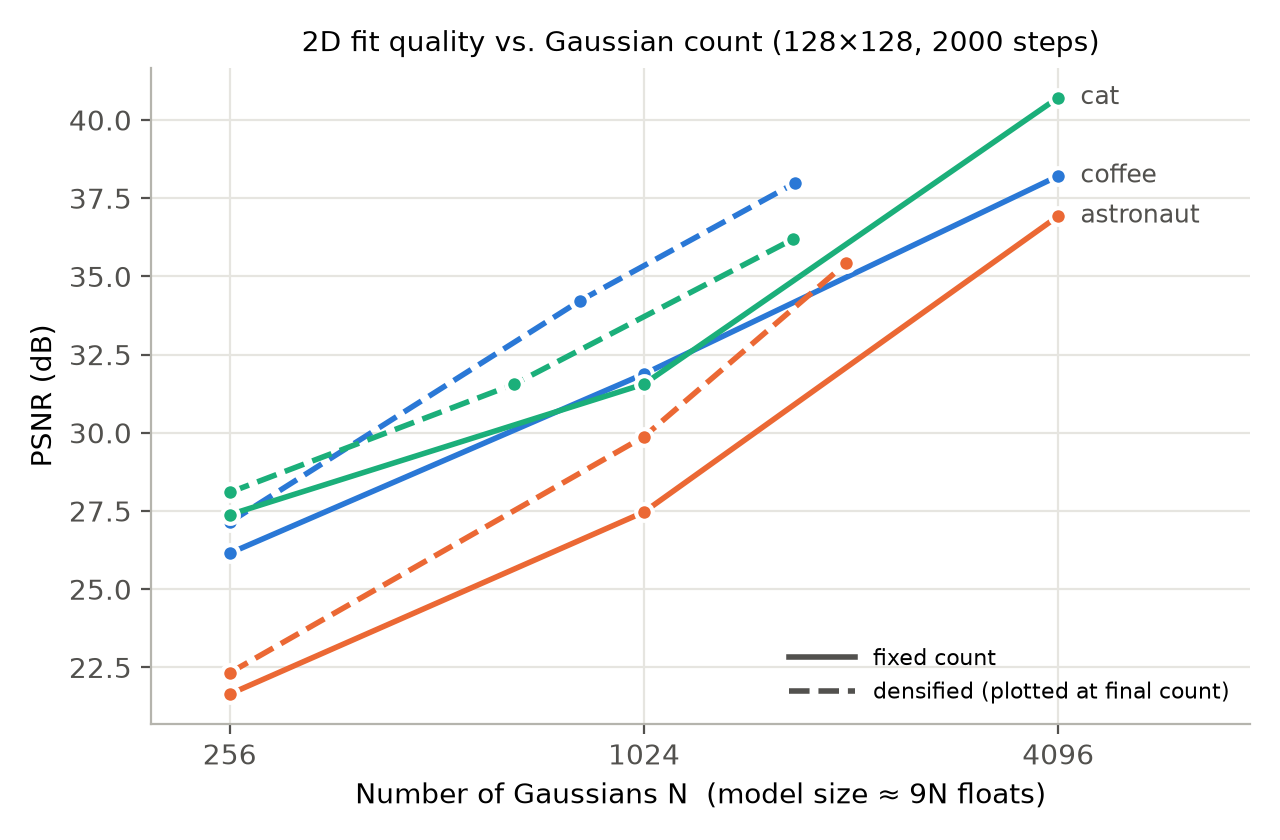
\includegraphics[width=0.72\textwidth]{psnr_vs_n.png}
\caption{PSNR against $N$ (log scale). Solid: fixed count (Table~\ref{tab:p5}). Dashed: densified runs, plotted at the count they actually ended with.}
\label{fig:p5}
\end{figure}

\paragraph{Astronaut needs the most Gaussians,} and is the lowest curve at every $N$, $4$--$6\dB$ behind the others at 256 and 1024. Its difficulty is structure rather than texture: flag stripes, the white suit against a black background, and lettering are long, sharp, high-contrast edges. A Gaussian has a soft profile, so representing an edge takes a row of small Gaussians along it, and every pixel the edge is wrong on costs a large squared error.

\paragraph{Coffee is the smooth case.} Large flat regions (saucer, table, coffee surface) are covered by a few large Gaussians, so it does well at low $N$. Its curve flattens toward 4096 because the remaining error is concentrated in a few sharp edges, the cup rim and the spoon.

\paragraph{Cat is easier than its frequency content suggests.} I expected the fur to be the hardest target, but at $128\times128$ it is the best at 4096 and close to coffee below that. Two reasons. Resizing from 256 to 128 removes the finest fur strands before fitting starts. And what remains is mostly low-contrast texture: the error is spread over many pixels but each error is small, which PSNR penalizes gently, while the high-contrast features (eyes, nose) are compact. I expect cat would fall behind at its native resolution. The steep jump from 1024 to 4096 also reflects that $N=4096$ is barely compression: $9N=36{,}864$ stored values against $49{,}152$ raw pixel values, about one Gaussian per four pixels, at which point the frequency content of the image matters much less.

\paragraph{Densified curves.} Densification is ahead at every matched count (all three images at 256, astronaut at 1024). With a fixed threshold, though, growth stalls once the fit is good: coffee and cat stopped at 827 and 663 of 1024, and all three 4096 runs stopped between 1688 and 2014. Even so, densified coffee reaches $37.99\dB$ with 1699 Gaussians against $38.21\dB$ for 4096 fixed ones, nearly the same quality with 41\% of the Gaussians. A top-$k$ fallback would force every run to its budget.

\section*{P7. 3D reconstruction}

\paragraph{Setup.} 4000 Gaussians, initialized exactly as in the handout: centers uniform in $[-1.5,1.5]^3$, isotropic scale $0.08$, identity quaternion, gray color, opacity $\approx0.12$. Each step picks a random training view, projects every Gaussian (P6: mean through the pinhole, covariance through $J R_{wc}\Sigma R_{wc}^\top J^\top$), skips Gaussians within $0.2$ of the camera plane, sorts the rest by camera depth $z_c$ nearest first, and composites with the tiled renderer. Following 3DGS, $0.3\,\mathrm{px}^2$ is added to each projected covariance so no splat is thinner than about a pixel. Training took 137\,s.

\paragraph{Result.} Mean PSNR over the 44 training views is $\mathbf{23.67\dB}$ (mean of per-view PSNR). The spheres are in the right places with the right colors, but soft, and the background is a noisy haze crossed by dark streaks (Figure~\ref{fig:p7}). Most Gaussians end near their initial opacity (median $0.11$); at lr $10^{-2}$ an opacity logit moves slowly, so the spheres are built from many faint blobs, and the bulk of the Gaussians drift outward (median $\|\mu\|=1.75$) to paint the background.

\begin{figure}[H]
\centering
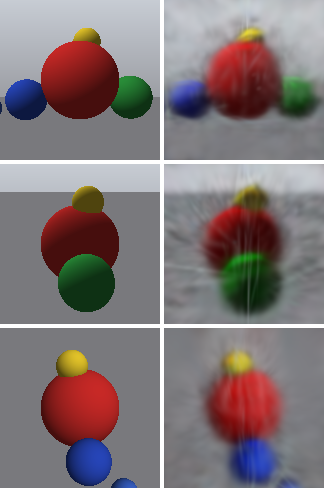
\includegraphics[width=0.36\textwidth]{p7_train.png}
\caption{Training views 000, 015, 033: ground truth (left) and the plain 4000-Gaussian fit (right).}
\label{fig:p7}
\end{figure}

\section*{P8. Densification in 3D}

\paragraph{What changed and what stayed the same.} The clone/split/prune logic and the Adam bookkeeping are the same code as P4; I generalized \code{densify} so the caller passes a size limit in its own units and a function returning each Gaussian's rotation matrix. What changed: means and scales are 3D and split offsets are sampled in 3D, $\mu+RSz$ with $R$ from the quaternion (clones and children copy the quaternion); the size threshold is $0.1$ world units instead of a fraction of the image; and the score is the world-space position gradient, averaged over the random cameras since the last pass. Passes run every 100 steps until step 1200, starting from 1000 Gaussians with a 4000 budget and threshold $10^{-4}$ (more than half of the Gaussians exceed it early in training, fewer later).

\paragraph{Pruning needed an opacity reset.} The handout identifies pruning as what removes floaters, but the floaters in the P7 fit sit around opacity $0.1$, twenty times the $0.005$ threshold, and a first densified run pruned nothing. So I added the 3DGS paper's opacity reset: every 400 steps (at 400 and 800) every opacity is capped at $0.01$ and Adam's opacity moments are cleared. Gaussians that the training views need grow back; haze that only explains individual views stays faint and can be pruned.

\begin{table}[H]
\centering
\begin{tabular}{lrrr}
\toprule
run & $N$ & train PSNR & held-out PSNR \\
\midrule
plain (P7) & 4000 & 23.67 & 16.43 \\
densified & 4000 & 23.82 & \textbf{18.76} \\
\midrule
\multicolumn{4}{l}{\emph{ablations}} \\
densified, no opacity reset & 4000 & 24.87 & 15.91 \\
densified, prune threshold $0.01$ & 3969 & 23.84 & 18.58 \\
\bottomrule
\end{tabular}
\caption{3D fits, 1500 steps each. Two identical runs differ by about $0.2\dB$ held-out (MPS is not deterministic).}
\label{tab:p8}
\end{table}

\begin{figure}[H]
\centering
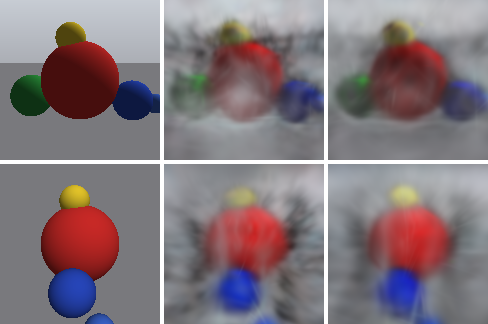
\includegraphics[width=0.54\textwidth]{p8_heldout.png}
\caption{Held-out views 002 and 007. Left to right: ground truth, plain fit, densified fit. The dark streaks (floaters) of the plain fit are mostly gone.}
\label{fig:p8}
\end{figure}

\paragraph{Result.} At the same count, the densified fit gains $2.3\dB$ on held-out views while training PSNR is essentially unchanged (Table~\ref{tab:p8}), and most of the floaters are visibly gone (Figure~\ref{fig:p8}). The ablations show where the gain comes from. Densifying \emph{without} the reset overfits more than the plain fit: higher training PSNR, lower held-out PSNR, because the new Gaussians are spent explaining individual views. The reset is what removes the floaters, by making every Gaussian re-earn its opacity against all views. Pruning itself removed nothing at the $0.005$ threshold, and raising the threshold to $0.01$ removed only 14 Gaussians and changed nothing beyond run-to-run noise. In a 1500-step schedule, then, the reset does the work by turning floaters nearly transparent, not by deleting them; a longer schedule would give the faint ones time to fall below the threshold.

\section*{P9. Novel-view evaluation}

\begin{table}[H]
\centering
\begin{tabular}{lrrr}
\toprule
held-out elevation & $5^\circ$ & $25^\circ$ & $45^\circ$ \\
\midrule
plain     & 14.74 & 17.54 & 17.02 \\
densified & 17.65 & 17.94 & 20.71 \\
\bottomrule
\end{tabular}
\caption{Mean held-out PSNR (dB) over the four views at each elevation. Training orbits are at $-5^\circ$, $15^\circ$, $35^\circ$, $55^\circ$.}
\label{tab:p9}
\end{table}

\paragraph{Held-out vs.\ training.} Held-out PSNR is $16.43\dB$ for the plain fit against $23.67\dB$ on training views, a $7.2\dB$ gap; for the densified fit it is $18.76$ against $23.82\dB$, a $5.1\dB$ gap. The gap is the part of the training fit that is memorization rather than reconstruction.

\begin{figure}[H]
\centering
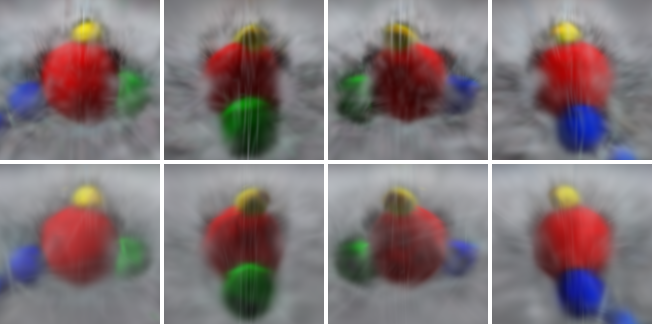
\includegraphics[width=0.8\textwidth]{p9_orbit.png}
\caption{Orbit at $25^\circ$ elevation, between the training orbits, azimuth $0^\circ$, $90^\circ$, $180^\circ$, $270^\circ$. Top: plain fit; bottom: densified fit. The full 36-frame orbits are \code{results/3d/plain/orbit.gif} and \code{results/3d/densify/orbit.gif} in the repository.}
\label{fig:orbit}
\end{figure}

\paragraph{Where it breaks down.}
\begin{itemize}
\item \textbf{The background} is the largest error. The ground truth has a sharp horizon between a light sky and a dark floor that extends to infinity. Gaussians near the origin cannot represent anything at infinity consistently, so each training view gets its own painted haze, which is wrong from any other angle. This is why the $5^\circ$ views, where the horizon crosses the frame, are worst (Table~\ref{tab:p9}), and the $45^\circ$ views, which see mostly uniform floor, are best for the densified fit.
\item \textbf{Floaters}: the dark streaks of the plain fit are elongated, faint Gaussians at wrong depths that help some training views and cut across novel ones. The opacity reset removes most of them (Figure~\ref{fig:p8}).
\item \textbf{Thin vertical needles} remain in the orbit (Figure~\ref{fig:orbit}). The training cameras lie on only four elevation rings, so a Gaussian stretched vertically is seen nearly end-on or blurred into the spheres from most training views, and little in the loss penalizes the stretch. From the $25^\circ$ orbit it shows up as a bright line.
\item \textbf{Softness everywhere.} At lr $10^{-2}$ opacities grow slowly, so solid spheres are approximated by many semi-transparent blobs, and their edges blur. The per-parameter learning rates used by 3DGS (much higher for opacity, much lower for position) would likely sharpen this; I kept the handout's single learning rate so the P7 result matches the specification.
\end{itemize}

\end{document}
